\documentclass{article}
\usepackage[svgnames]{xcolor}
\usepackage[a0paper,landscape,margin=3cm]{geometry}
\usepackage[utf8]{inputenc}
\usepackage[sorting=nyt,backend=biber,style=authoryear,block=par]{biblatex}
\usepackage{anyfontsize}
\usepackage{tikz}
\usepackage{mathpazo}
\usepackage{multicol}
\usepackage{tikz}
\usepackage{graphicx}
\usepackage{graphicx}
\usepackage[inkscapeformat=png]{svg}
\usetikzlibrary{matrix,fadings,arrows,trees,calc,positioning,decorations,automata,fit,backgrounds}
\usepackage{blindtext}
\usepackage[inkscapeformat=png]{svg}
\usepackage{booktabs}
\pagecolor{red!5}

\columnsep=50pt
% \columnseprule=2pt
\graphicspath{ {images/} }
\addbibresource{References.bib}

\renewcommand{\section}[1]{
    \begin{center}
        \begin{tikzpicture}
            \draw node[fill=white!10, text width=0.97\linewidth, text centered, inner sep=10pt, rounded corners=5pt, draw=red!80]
            {\textbf{#1}};
        \end{tikzpicture}
        
    \end{center}

}

\renewcommand{\subsection}[1]{
    \begin{center}
        \begin{tikzpicture}
            \draw node[fill=white!10, text width=0.97\linewidth, text centered, inner sep=10pt, rounded corners=5pt, draw=red!30]
            {\textbf{#1}};
        \end{tikzpicture}
        
    \end{center}

}

\begin{document}
    \fontsize{55}{65}
    \selectfont
     \begin{tikzpicture}
            
        \node[inner sep=0pt] (logo) {\includesvg{SRH_Bildung.svg}}; 
        \draw node[text width=0.87\linewidth,text centered,rounded corners=5pt,inner sep=30pt,right=100pt of logo] (title){
            {Application of Natural Language Processing in an E-commerce industry}\\[0.5cm]
            \fontsize{50}{55}
            \selectfont
            {Predicting multilevel product category} \\[1cm]  
            \fontsize{40}{50}
            \selectfont
            Shoney Arickathil, Prof. Dr. Gerd Moeckel \\[0.5cm]
            \fontsize{50}{50}
            \selectfont
            Applied Computer Science, SRH Hochschule, Heidelberg
            };
    \begin{scope}[on background layer]
        \node [fill=Red!10, fit={(logo) (title)}] {};
    \end{scope}

\end{tikzpicture}
\vspace{1cm}
\begin{multicols}{3}

   
    \fontsize{30}{40}
    \selectfont
    \section{Introduction}
    Ever increasing demand of online platforms trending online shopping huge number of products for online sales  need to add category for the products Un matching product taxonomy from various source. Existing taxonomy unsupervised learning model need of the hour to create an AI model to predict the category tree in which the product belongs to based on the product features such as description, manufacture.
    
 
    \section{Problem statement and objective}
    Suppliers and manufactures provide the product details which must be analyzed and fit into the existing vocabular of the product category taxonomy. Make deployment ready products taxonomy. If a supplier name a certain product category as "Engine oil" and the category already existing is "Motor Oil". In such case importing the category from the supplier may lead to having two categories at same level. Imagine this issue with thousands of products solds on the ecommerse website. The ecomerse webiste will need to manage many categories. This paper researched on implementation of a text based classification model for predicting the category of the product based on product features. 

    \begin{multicols}{2}
        \section{Tools and Technologies}
            \includesvg{PyTorch_logo_black.svg} \\
            Pytorch  \parencite{Paszke.03122019} is a machine learnning library which provides Pythonic programming style. The open-source Python ecosystem packages like NumPy, SciPy and Pandas fulfills most of the numerical analysis needs of research.  Python provides vast repositories of libraries to handle data preprocessing, statistical analysis and plotting. 

            Pytorch performs execution of dynamic tensors computation with automatic differentiation for efficient gradient based optimization. 
            \columnbreak     

        \section{Research questions}
        \begin{enumerate}
            \item How Natural Language Processing (NLP) can be applied in ecommerse industry?
            \item Which neural network architecture is suitable for text based classification model?
            \item What are the steps involved for preprocessing text to extract features from the document?
            \item  How to get better results with better shaped network? Evaluate neural network performance based on confusion matrix.
        \end{enumerate}
     
    \end{multicols}

    \section{Evaluation and Results}
    \begin{enumerate}
        \item Preprocessing of the product and category data frame is performed, which involves step:-
        \begin{enumerate}
            \item Normalization of text: lowercase, perform Tf-Idf, ngram vectorization to extract text.
            \item To change \"A to A, the Normal form D (NFD) should be applied which translates each character into its decomposed form.
            \item Use Beautiful Soup a Pyhon library for pulling data out of HTLM and XML.
        \end{enumerate}
        \item The developed text based classification model successfully preditcs the product taxonomy based on the product features.
        \item The time required to analyze the product details before it is ready deploy is reduced. As manual work of defining the product taxonomy is automated.  
        \item Better shaped neural network architecture is developed. 
        
    \end{enumerate}
    \subsection{Table: Before and After normalization}
    \begin{center}
        \begin{tabular}{lll}
            \toprule 
                    &\textbf{Name} & \textbf{Category} \\ 
            \midrule
            \textbf{Before}&VAICO V10-4245 Stoßdämpfer & Stoßdämpfer \\
            \textbf{After}&vaico stoßdampfer & stoßdampfer \\
        
            \bottomrule
        \end{tabular}
        
    \end{center}

    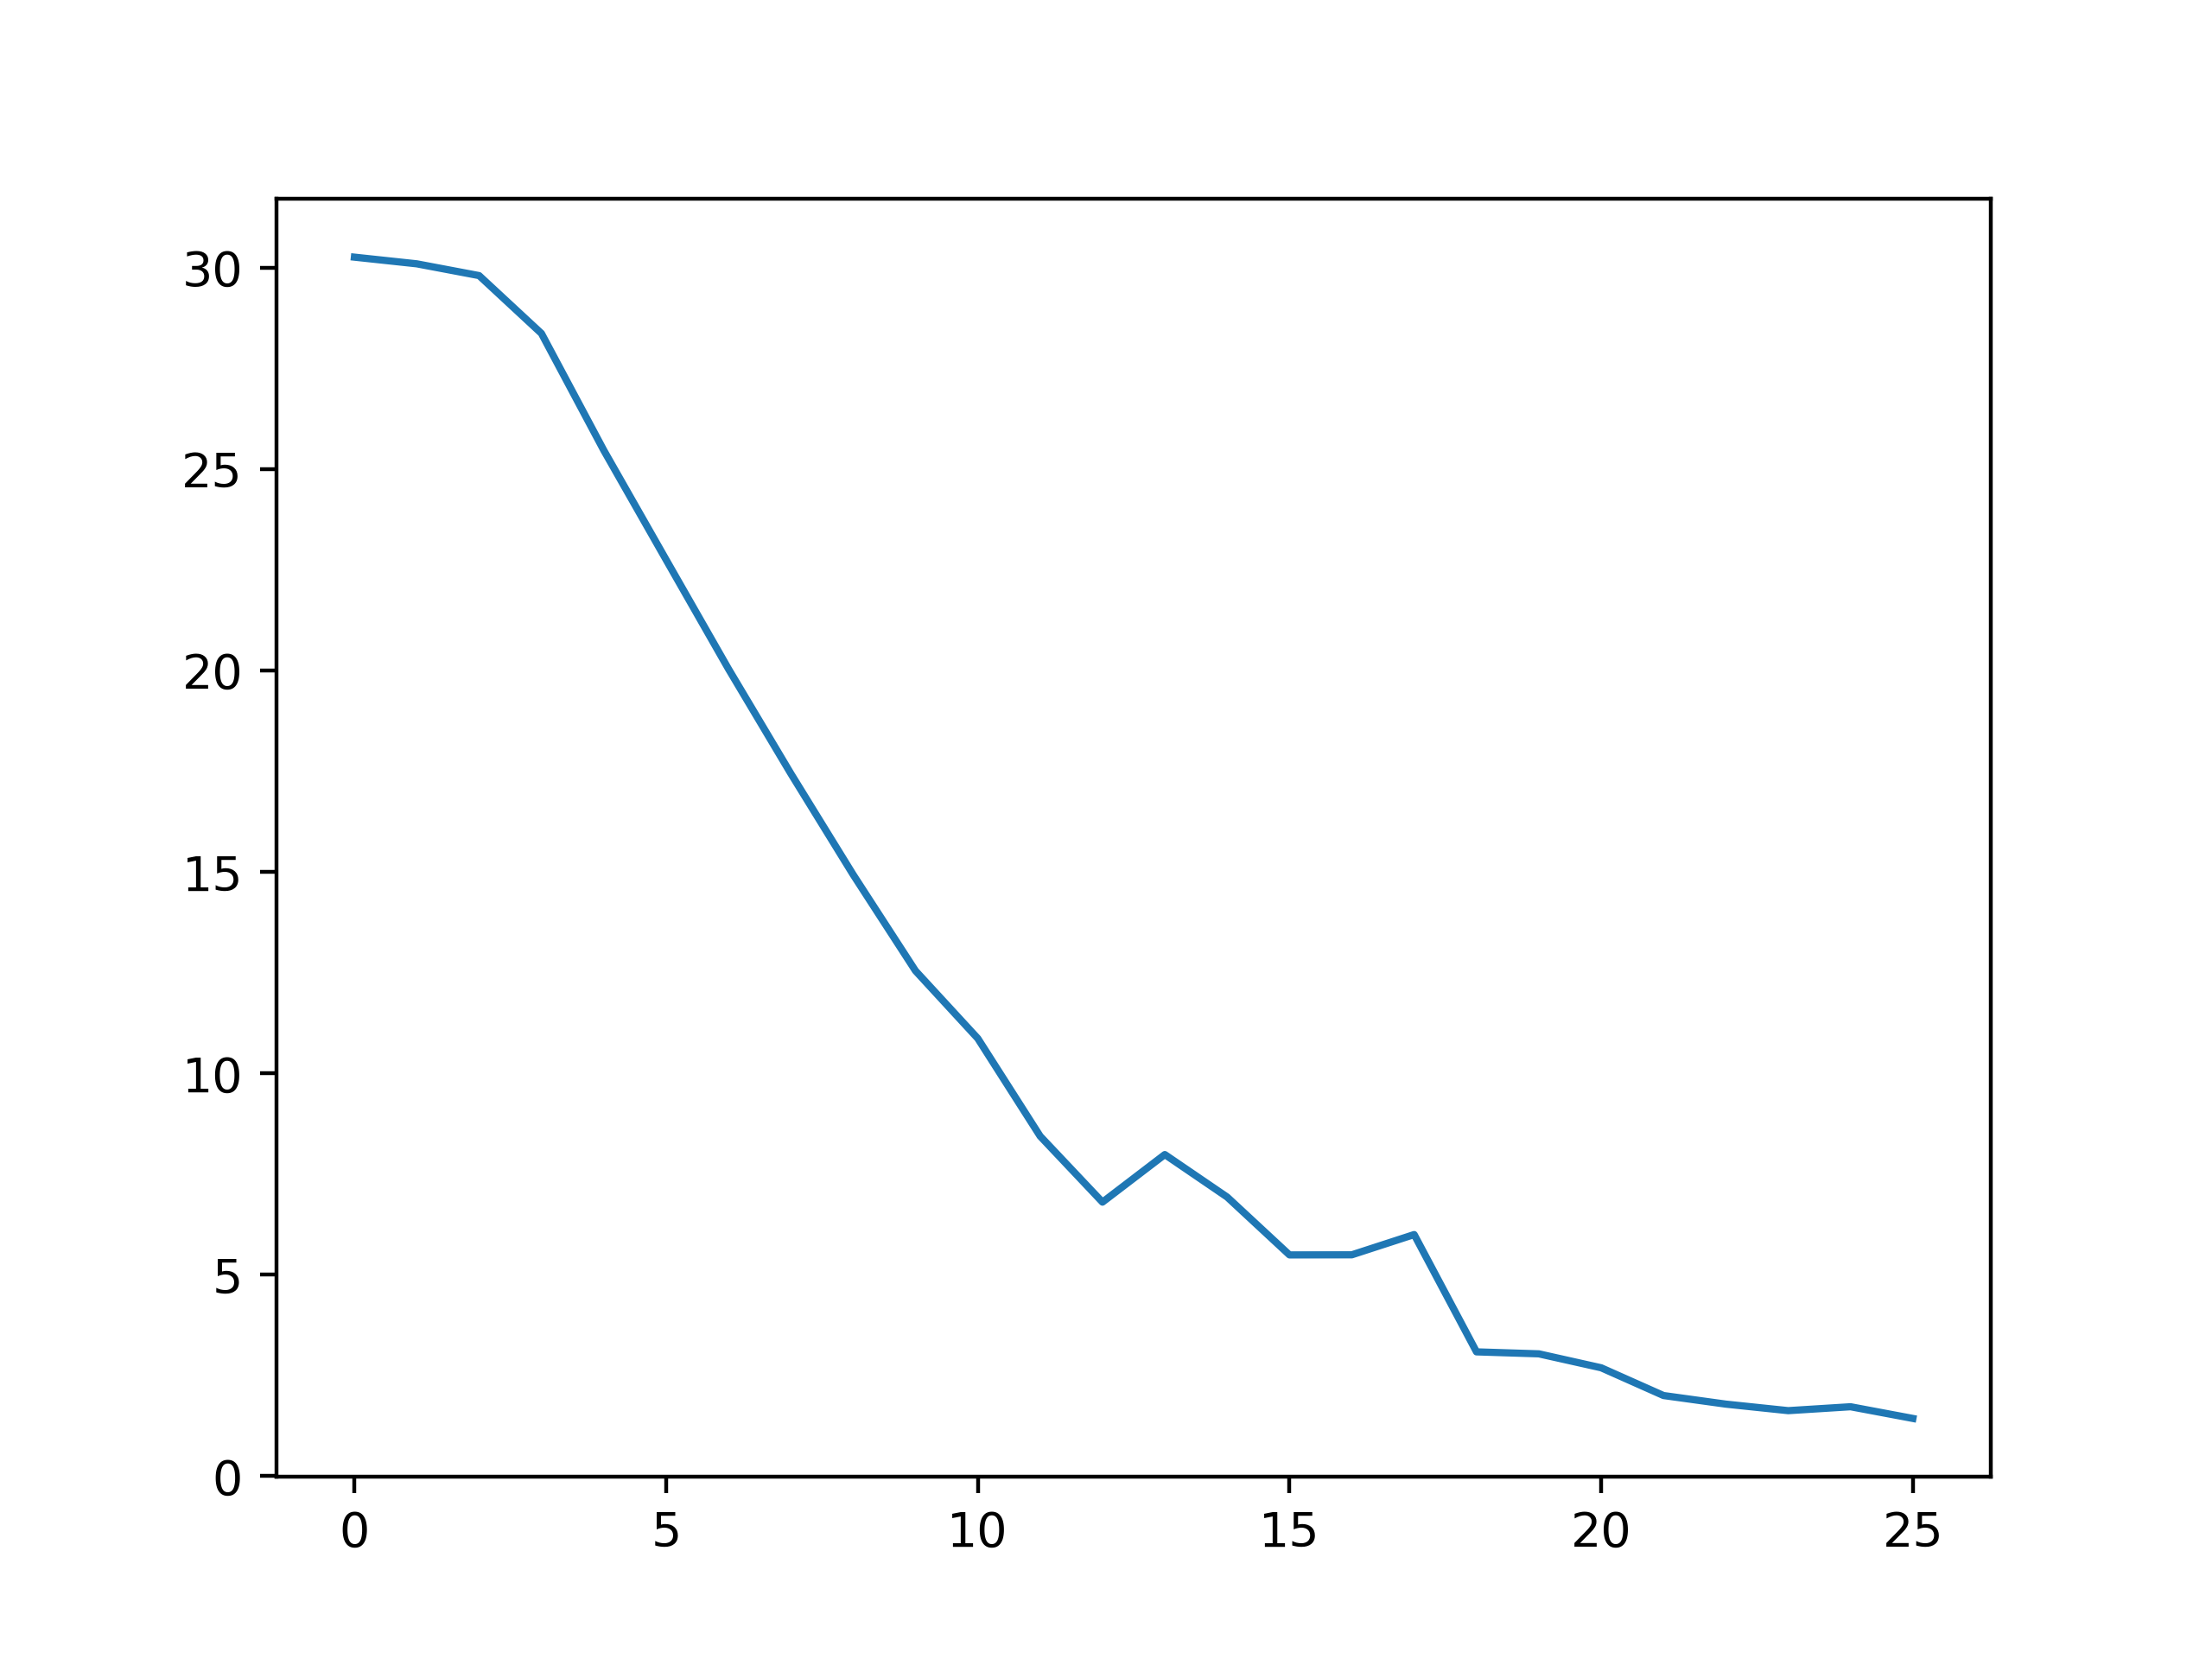
\includegraphics{histogram}

          
    
\end{multicols}

% \printbibliography


\end{document}